\subsection{A Cluedo társasjáték}
A Cluedo nevű társasjáték egy olyan logikai detektívjáték, ahol azt kell kideríteni,
hogy ki ölte meg a játék színteréül szolgáló ház tulajdonosát. A gyilkosság idejében
hat vendég tartózkodott a házban, így mind a hatan gyanúsítottak lettek.

A házban kilenc helység található, valamint hat lehetséges gyilkos fegyvert találtak
a detektívek. A játékosok egy-egy gyanúsított bőrébe bújva próbálják meg kideríteni,
hogy melyik helységben, ki és mivel követte el a gyilkosságot.

\subsubsection{A játék tartozékai}
\begin{itemize}
  \item ház alaprajz játéktábla
  \item detektív jegyzettömb
  \item 6 karakter bábu és nyomkártya
  \item 6 gyilkos fegyver és nyomkártya
  \item 9 szoba nyomkártya
  \item 2 dobókocka
  \item boríték, a gyilkosság nyomkártyáinak
\end{itemize}

\begin{figure}[h!]
  \centering
  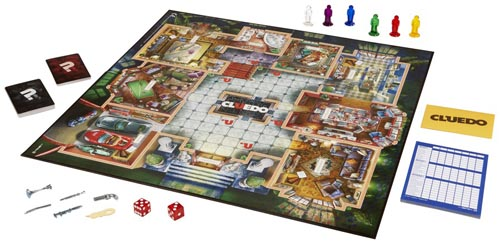
\includegraphics[width=0.9\textwidth]{user-documentation/images/cluedo.jpg}
  \caption[]{Egy modern Cluedo játéktábla és tartozékai\footnotemark}
\end{figure}
\footnotetext{Kép forrása: \url{http://images.esellerpro.com/2489/I/108/074/7/38712_2.jpg} (2015. 09. 19.)}

\subsubsection{A játék menete}
A játékmenet a történet után nagyon egyszerű: a játéktér a ház alaprajza, melyben
a játékosok kockadobás segítségével közlekedhetnek egyik helységből a másikba.

Minden karakternek, gyilkos fegyvernek és szobának van egy kártyája. A játék elején
ezekből a kártyákból a játékosok kihúzzák, hogy ki, hol és mivel gyilkolt, ügyelve,
hogy senki ne láthassa meg a kihúzott lapokat. A maradék lapok pedig keverés után
kiosztásra kerülnek a játékosok között.

A játék körökre osztott, a játékosok egymás után sorban következnek. Egy kör akkor
ér véget, amikor újra az első játékosra kerül a sor. Egy körben minden játékos
dob a kockával, lép, és ha bejutott egy szobába, akkor gyanúsíthat.\\
A gyanúsítás során a játékos megkérdezheti a következő játékostól, hogy az
aktuális szobában X gyilkolt-e Y fegyverrel (X egy karakter, Y egy gyilkos eszköz).

Amennyiben a következő játékos rendelkezik valamelyik kártyával, akkor abból egyet
meg kell mutatnia szigorúan csakis annak a játékosnak, aki kérdezett tőle, majd
az ő köre következik.

A játékot az nyeri, aki a leghamarabb ki tudja találni, hogy mi volt az a három
lap, amit az elején kihúztak. Ha valaki rájött a megoldásra, akkor a pálya közepére
kell mennie, ahol megvádolhatja a gyilkos személyt, a gyilkos eszköz és a helyszín
megnevezésével. Ekkor ő megnézheti azokat a lapokat, amiket a játék elején kihúztak
és amennyiben igaza volt, a játék véget ért és ő nyert. Ellenben, ha tévedett,
akkor kiesett a játékból és saját lapjait fel kell fednie a többi játékos előtt,
majd a játék addig folytatódik, amíg nem érkezik helyes megfejtés, vagy amíg csak
egy játékos marad játékban. Ebben az esetben senki nem nyerte meg a játékot.

\clearpage
